% !TEX encoding = UTF-8 Unicode
\documentclass[a4paper]{article}

\usepackage{color}
\usepackage{url}
\usepackage[T2A]{fontenc} % enable Cyrillic fonts
\usepackage[utf8]{inputenc} % make weird characters work
\usepackage{graphicx}
\usepackage{tcolorbox}

\usepackage[english,serbian]{babel}
%\usepackage[english,serbianc]{babel} %ukljuciti babel sa ovim opcijama, umesto gornjim, ukoliko se koristi cirilica

\usepackage[unicode]{hyperref}
\hypersetup{colorlinks,citecolor=green,filecolor=green,linkcolor=blue,urlcolor=blue}

\usepackage{listings}

%\newtheorem{primer}{Пример}[section] %ćirilični primer
\newtheorem{primer}{Primer}[section]

\definecolor{mygreen}{rgb}{0,0.6,0}
\definecolor{mygray}{rgb}{0.5,0.5,0.5}
\definecolor{mymauve}{rgb}{0.58,0,0.82}

\lstset{ 
  backgroundcolor=\color{white},   % choose the background color; you must add \usepackage{color} or \usepackage{xcolor}; should come as last argument
  basicstyle=\scriptsize\ttfamily,        % the size of the fonts that are used for the code
  breakatwhitespace=false,         % sets if automatic breaks should only happen at whitespace
  breaklines=true,                 % sets automatic line breaking
  captionpos=b,                    % sets the caption-position to bottom
  commentstyle=\color{mygreen},    % comment style
  deletekeywords={...},            % if you want to delete keywords from the given language
  escapeinside={\%*}{*)},          % if you want to add LaTeX within your code
  extendedchars=true,              % lets you use non-ASCII characters; for 8-bits encodings only, does not work with UTF-8
  firstnumber=1000,                % start line enumeration with line 1000
  frame=single,	                   % adds a frame around the code
  keepspaces=true,                 % keeps spaces in text, useful for keeping indentation of code (possibly needs columns=flexible)
  keywordstyle=\color{blue},       % keyword style
  language=Python,                 % the language of the code
  morekeywords={*,...},            % if you want to add more keywords to the set
  numbers=left,                    % where to put the line-numbers; possible values are (none, left, right)
  numbersep=5pt,                   % how far the line-numbers are from the code
  numberstyle=\tiny\color{mygray}, % the style that is used for the line-numbers
  rulecolor=\color{black},         % if not set, the frame-color may be changed on line-breaks within not-black text (e.g. comments (green here))
  showspaces=false,                % show spaces everywhere adding particular underscores; it overrides 'showstringspaces'
  showstringspaces=false,          % underline spaces within strings only
  showtabs=false,                  % show tabs within strings adding particular underscores
  stepnumber=2,                    % the step between two line-numbers. If it's 1, each line will be numbered
  stringstyle=\color{mymauve},     % string literal style
  tabsize=2,	                   % sets default tabsize to 2 spaces
  title=\lstname                   % show the filename of files included with \lstinputlisting; also try caption instead of title
}

\begin{document}

\title{TargetSearch algoritam kao vrsta pretrage alata KLEE\\ \small{Seminarski rad u okviru kursa\\Verifikacija softvera\\ Matematički fakultet}}

\author{Luka Milošević, Filip Jovašević\\ lukamilosevic11@gmail.com, filip.jovasevic96@gmail.com}

%\date{9.~april 2015.}

\maketitle

\abstract{
Cilj ovog rada je da svim zainteresovanim osobama koji žele da znaju nešto više iz oblasti verifikacije i validacije softvera približi pojam i značenje simboličkog izvršavanja programa. Čitajući rad, čitalac će se upoznati sa alatom KLEE koji služi za simobličko izvršavanje programa. Pored pretraga koje ovaj alat podrazumeva detaljno će biti predstavljena nova pretraga koju smo mi, kao autori ovog rada, implementirali i nazvali TargetSearch. }

\tableofcontents

\newpage

\section{Uvod}
\label{sec:uvod}
Validacija i verifikacija softvera predstavljaju dve bitne oblasti čija je namena briga o kvalitetu softvera. Validacija proverava da li specifikacija zadovoljava korisničke potrebe, dok verifikacija proverava da li softver zadovoljava specifikaciju. Zbog teme ovog rada, više pažnje ćemo posvetiti verifikaciji. \\
Osnovne tehnike verifikacije softvera su: 
\begin{itemize}
    \item Dinamička verifikacija $\rightarrow$ proveravanje ispravnosti koda u fazi izvršavanja, najčešće testiranjem
    \item Statička verifikacija $\rightarrow$ proveravanje ispravnosti koda bez njegovog izvršavanja formalnim metodama ili ručnim proverama i pregledima koda
\end{itemize}
Što se tiče formalnih metoda kao vrste statičke verifikacije, ideja je da se one automatizuju. Ovo jeste moguće ali se ne može garantovati utvrđivanje ispravnosti proizvoljnog programa potpuno precizno \cite{Verifikacija}. U automatske formalne metode spadaju:
\begin{itemize}
    \item Simboličko izvršavanje
    \item Proveravanje modela
    \item Apstraktna interpretacija
\end{itemize} 
Kroz rad će detaljnije biti opisano simboličko izvršavanje kao i strategija obilaska puteva pod nazivom TargetSearch implementirana u softverskom alatu KLEE. Ova pretraga je implementirana od strane naših kolega sa fakulteta \cite{git}, a u ovom radu će biti opisano na koji način smo je mi unapredili. 

\section{Simboličko izvršavanje programa}
Simboličko izvršavanje programa predstavlja izvršavanje programa sa simbolima, tačnije praćenje simboličkih stanja umesto konkretnih ulaza. Ovom tehnikom se izvršava mnogo putanja istovremeno i svaka putanja simulira veliki broj testova jer se razmatraju svi ulazi koji prolaze kroz tu putanju. Tehnika je nastala sedamdesetih godina prošlog veka, ali je tek od 2005. godine omogućena praktična primena simboličkog izvršavanja. Alati koji su prvo bili korišćeni su DART I EXE. Neki od alata koji se koriste i danas su: SAGE, CUTE, Cloud9, Kleenet i KLEE o kojem će biti nešto više reči u narednoj sekciji. Simboličko izvršavanje u toku svog rada gradi stablo izvršavanja \ref{fig:stablo}. Ono se sastoji od svih putanji programa. Uslov putanje (path condition) koji je označen na slici predstavlja formulu (bez kvantifikatora) koja sadrži sve odluke koje su do tog trenutka donete \cite{Simbolicko}. Za obilazak puteva koriste se različite strategije kao što su DFS, BFS, Random Path, izvršavanje vođeno pokrivenošću koda itd. O njima neće biti reči u ovom radu. U sekciji \ref{sec:Target} možete naći sve informacije o strategiji obilaska kojoj smo mi posvetili pažnju. 

\begin{figure}
    \centering
    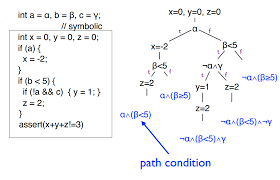
\includegraphics[scale=1.0]{stabloIzvrsavanja.png}
    \caption{Stablo izvršavanja}
    \label{fig:stablo}
\end{figure}
\includegraphics

\newpage
\section{KLEE}	
KLEE je simbolička virtuelna mašina koja je izgrađena koristeći LLVM infrastrukturu kompajlera kao osnovu. Omogućava automatsko generisanje testova koji postižu visoku pokrivenost nad različitim skupom kompleksnih programa \cite{kleeDok}. Kao što je pomenuto u prethodnoj sekciji, EXE je bio jedan od prvih alata za simboličko izvršavanje. Baš taj alat koji su napravili Cristian Cadar i Dawson Engler je kasnije preimenovan u KLEE. Zadatak ovog alata je da u kodu pronađe bagove i generiše test primere za njih. Do sada, KLEE je pronašao veliki broj problema u softveru otvorenog koda \cite{kleeRad}. Da biste mogli da koristite KLEE, neophodno je prvo da vaš program prevedete u bajtkod. To možete postići sledećom komandom:
\begin{tcolorbox}[title={Prevođenje programa u bajtkod}]
    clang-6.0 -emit-llvm -c -g ime\_programa.c
\end{tcolorbox}
Nakon što je program preveden u bajtkod, možete koristiti klee. Jedan jednostavan primer bi bio:
\begin{tcolorbox}[title={Primer korišćenja KLEE alata}]
    klee ime\_programa.bc
\end{tcolorbox}
KLEE nudi mogućnost odabira strategije obilaska puteva. U sekciji \ref{sec:Target} možete videti primer poziva alata KLEE gde je za strategiju obilaska puteva odabrana strategija target-searcher \ref{lst:targetSearch}.
\newpage

\section{TargetSearch}\label{sec:Target}
TargetSearch je algoritam koji predstavlja unapređenje već pomenutog algoritma. Osnovna ideja je da se omogući pretraga na nivou funkcije i da različite funkcije mogu da se obilaze različitim načinom pretrage. Tačnije, neophodno je da korisnik definiše vrstu pretrage, a nakon nje i funkcije koje će biti izvršene tom vrstom. Korisnik je u mogućnosti da definiše više od jedne vrste pretrage, a maksimalno pet i za svaku od njih navede imena funkcija koje želi da izvrši tom vrstom. Mogućnost da se definiše i do pet pretraga predstavlja prvo bitno unapređenje u odnosu na postojeći rad. Vrste pretraga koje se mogu odabrati su:
\begin{itemize}
    \item DFS search $\rightarrow$ --target-dfs komanda
    \item BFS search $\rightarrow$ --target-bfs komanda
    \item Random search $\rightarrow$ --target-rs komanda
    \item Random-path search $\rightarrow$ --target-rps komanda
    \item Weighted-random search $\rightarrow$ --target-wrs komanda
\end{itemize}
Ispod možete videti kako izgleda poziv našeg algoritma na veštačkom primeru.
\begin{tcolorbox}[label={lst:targetSearch}, title={Primer korišćenja TargetSearch pretrage}]
klee --search=target-searcher --target-bfs=f1,f2, f3 --target-dfs=f4 --target-rps=f5, f6 program.bc
\end{tcolorbox}
Nakon komande ${search}$ navodimo vrstu pretrage koju želimo da koristimo. U ovom slučaju smo odabrali našu vrstu pretrage. Da bismo definisali koje funkcije želimo da izvršimo kojom vrstom pretrage, neophodno je da te funkcije navedemo u komandnoj liniji. U ovom konkretnom slučaju, želimo funkcije $f1$, $f2$, $f3$ da izvršimo $bfs$ pretragom, funkciju $f4$ $dfs$ pretragom, a funkcije $f5$ i $f6$ $random-path$ pretragom.\\
Sve ostale funkcije koje se nalaze u kodu koji testiramo će u ovom konkretnom slučaju biti pretražene bfs pretragom. Razlog za ovakvo ponašanje je taj što smatramo da ukoliko je najveći broj funkcija koje smo naveli izvršen $bfs$ pretragom($bfs$ $\rightarrow$ tri funkcije, $dfs$ $\rightarrow$ jedna funkcija, $rps$ $\rightarrow$ dve funkcije), velika je verovatnoća da će i preostalim funkcijama najviše pogodovati ta vrsta pretrage.\\
Važno je i napomenuti da je u slučaju ${Weighted-random}$ pretrage moguće dodati i željenu heuristiku, ali nije neophodno. \\
Poslednji argument komandne linije je program koji testiramo koji je prethodno preveden u bajtkod.\\
Kroz sekcije \ref{subsec:impl} i \ref{subsec:rez} biće prikazano na koji način su sve ove mogućnosti postignute kao i upoređivanje rezultata našeg algoritma u odnosu na rezultate korišćenja pretraga koje nudi alat KLEE.
\newpage
\subsection{Implementacija}\label{subsec:impl}
U ovom odeljku će detaljnije biti objašnjeno kako je algoritam konstruisan, to jest koji su fajlovi izmenjeni i koje su funkcionalnosti dodate. \\

Počećemo od fajla ``ExecutionState.h``. Ovde je bilo neophodno definisati kojim sve načinima pretrage može biti izvršeno neko stanje. Zato smo iskoristili tip $enum$ prilikom definisanja pet vrsti pretraga koje smo spominjali u sekciji \ref{sec:Target}.
\begin{lstlisting}
enum searcherType {sDFS,sBFS,sWRS,sRPS,sRandomSearcher,sNotDet};
\end{lstlisting}
Na primeru se može videti i oznaka \textit{sNotDet} koju do sada nismo spominjali jer nije važna za razumevanje algoritma već služi isključivo implementaciji.\\

Incijalizacija svih stanja na podrazumevanu vrstu pretrage je izvršena u fajlu ``ExecutionState.cpp``. Podrazumevanom pretragom se smatra ona pretraga koja je od strane korisnika dobila najveći broj funkcija, kao što smo to prethodno naveli.

``Interpreter.h`` fajlu je dodata virtualna funkcija koja za cilj ima da vrati sve funkcije koje je korisnik eksplicitno naveo želeći da ih izvrši navedenim vrstama pretrage.
\begin{lstlisting}
virtual const std::unordered_map<std::string, searcherType>& getAllTargetFunctions() = 0;
\end{lstlisting}
Osim toga, kao argument funkcije \textit{runFunctionAsMain} dodat je tip pretrage da bismo mogli da izvršimo inicijalizaciju koju smo malopre pomenuli. 
\begin{lstlisting}
virtual void runFunctionAsMain(llvm::Function *f,
                                 int argc,
                                 char **argv,
                                 char **envp,searcherType type,std::vector<bool>& ifSearchers) = 0;
\end{lstlisting}

Mogućnost da kao argumente komandne linije zadajemo vrste pretrage je implementirana u fajlu ``main.cpp`` 
\begin{lstlisting}[title={Definisanje imena pretrage za komandnu liniju}]
cl::opt<std::string>
  TargetFunctionDFS("target-dfs",cl::desc("Target Functions for DFS"),cl::init(""));
\end{lstlisting}
Ovde je implementirana još jedna bitna funkcionalnost, a to je manipulacija funkcijama koje je korisnik naveo. Ona je postignuta funkcijom \textit{processTargetFunction} koja popunjava matricu funkcijama koje je korisnik naveo korišćenjem funkcije \textit{fillTargetFunctions}
\begin{lstlisting}[title={Popunjavanje mape}]
    while(!targetFunction.empty()){
        int pos=targetFunction.find_first_of(',');
        std::string s = targetFunction.substr(0,pos);
        m_allTargetFunctions[s] = searchType;
        if(pos == -1)
            return;
        targetFunction=targetFunction.substr(pos+1);
    }
\end{lstlisting}

a zatim i određuje najučestaliju pretragu. 
\begin{lstlisting}[title={Određivanje najučestalije pretrage}]
    for(int i = sDFS; i < sNotDet; i++){
        if(nums[i] > mmax){
            mmax = nums[i];
            m_maxType = (searcherType)i;
        }
    }
\end{lstlisting}

Modifikovanjem fajla ``UserSearcher.cpp`` izvršeno je instanciranje TargetSearch klase. Razlika u odnosu na projekat koji unapređujemo je ta što se konstruktoru klase TargetSearch dodaje argument typeWRS za slučaj da korisnik želi neke funkcije da izvrši WeightedRandom pretragom.

Klasu čiju smo instancu malopre pomenuli smo morali negde i da definišemo. To smo uradili u fajlu ``Searcher.h``. Pomenuti argument za WeightedRandom pretragu ne mora da se navede, u tom slučaju podrazumevana vrednost je minDistUncovered. 
\begin{lstlisting}[title={TargetSearcher klasa}, label={lst:kod}]
class TargetSearcher : public Searcher{
      WeightedRandomSearcher::WeightType m_typeWRS;
      Executor &m_executor;
      
      DFSSearcher searcherDFS;
      BFSSearcher searcherBFS;
      RandomSearcher searcherRandomSearcher;
      WeightedRandomSearcher searcherWRS{m_typeWRS};
      RandomPathSearcher searcherRPS{m_executor};
      
      std::vector<Searcher*> choose;
  public:
      TargetSearcher(Executor& executor, std::vector<bool>& ifSearchers, WeightedRandomSearcher::WeightType typeWRS = WeightedRandomSearcher::MinDistToUncovered);
      ~TargetSearcher();
	  ExecutionState &selectState();
	  void update(ExecutionState *current,
			  const std::vector<ExecutionState*> &addedStates,
			  const std::vector<ExecutionState*> &removedStates);
	  bool empty() { return ((searcherDFS?searcherDFS->empty():true) 
                          && (searcherBFS?searcherBFS->empty():true) 
                          && (searcherRandomSearcher?searcherRandomSearcher->empty():true) 
                          && (searcherWRS?searcherWRS->empty():true) 
                          && (searcherRPS?searcherRPS->empty():true)); }
	  void printName(llvm::raw_ostream &os) {
		  os << "TargetSearcher\n";
	  }
  };
\end{lstlisting}

Drugo bitno unapređenje rada na koji referišemo je implementirano u fajlu ``Searcher.cpp``, jer se umesto imitacije pretraga koristi postojeća implementacija pretraga KLEE-a. 

\newpage
\begin{lstlisting}[title={Odabir sledećeg stanja}]
    ExecutionState &TargetSearcher::selectState(){

        if(searcherDFS && !searcherDFS->empty()){
            return searcherDFS->selectState();
        }else if(searcherBFS && !searcherBFS->empty()){
            return searcherBFS->selectState();
        }else if(searcherWRS && !searcherWRS->empty()){
            return searcherWRS->selectState();
        }else if(searcherRandomSearcher && !searcherRandomSearcher->empty()){
            return searcherRandomSearcher->selectState();
        }else if(searcherRPS && !searcherRPS->empty()){
            return searcherRPS->selectState();
        }
    }
\end{lstlisting}
Kao i u slučaju odabira sledećeg stanja, tako je i funkcija update pozivana za svaku pretragu posebno i tako je iskorišćena originalna implementacija.
\begin{lstlisting}[title={Update funkcija}]
        if(searcherDFS) searcherDFS->update(current,addedStatesDFS,removedStatesDFS);
        if(searcherBFS) searcherBFS->update(current,addedStatesBFS,removedStatesBFS);
        if(searcherRandomSearcher) searcherRandomSearcher->update(current,addedStatesRandomSearcher,removedStatesRandomSearcher);
        if(searcherWRS) searcherWRS->update(current,addedStatesWRS,removedStatesWRS);
        if(searcherRPS) searcherRPS->update(current,addedStatesRPS,removedStatesRPS);
\end{lstlisting}

Ovo unapređenje je implementirano tako što smo umesto čuvanja stanja u jednom vektoru(što je do sada bio slučaj jer je korišćena jedna pretraga) stanja čuvali u mapi sa vrstom pretrage kojom treba da budu obiđena. Neophodno je bilo da kao polja klase TargetSearcher dodamo pet željenih pretraga, što se može videti u kodu \ref{lst:kod}. 

Implementacija funkcije koja reaguje na svako pojavljivanje funkcije u kodu koja je navedena od strane korisnika napisana je u fajlu ``Executor.h``. U pitanju je funkcija \textit{ifTargetFunction} i ona ima za cilj da odredi kojoj pretrazi ta funkcija pripada.
\begin{lstlisting}[title={Provera kojoj pretrazi funkcija treba da pripada}]
   searcherType ifTargetFunction(const llvm::Function *f){
      if(!f){
		  return sNotDet;
	  }
	  std::string functionName=f->getName();
      auto type = allTargetFunctions.find(functionName);
      if(type != allTargetFunctions.end())
          return type->second;
      
      return sNotDet;
  }
\end{lstlisting}


``Executor.cpp`` je fajl u kojem je rešen problem prelaska jednog načina pretrage u drugi nad istim stanjem. Kao što smo već rekli, koristimo pet vektora i neophodno je postarati se da se trenutno stanje nalazi u pravom vektoru. Zahvaljući prethodno opisanoj funkciji, znamo u koji vektor treba da smestimo trenutno stanje.

\newpage
\begin{lstlisting}[title={Prebacivanje stanja u odgovarajući vektor}]
    searcherType method = ifTargetFunction(f);
    
    if(method != sNotDet && method != state.s){
        searcher->removeState(&state);
        state.s = method;
        searcher->addState(&state);
    }
\end{lstlisting}

\subsection{Rezultati}\label{subsec:rez}
Nakon što smo videli kako algoritam funkcioniše i na koji način smo to postigli, sada je red došao da ga uporedimo sa postojećim algoritmima KLEE-a. Fajl nad kojim smo vršili testiranje se sastoji od sedam funkcija. Svaka od tih funkcija je specijalno prilagođena određenim strategijama pretrage sa ciljem da se demonstrira moć našeg algoritma. U svakoj funkciji se nalazi greška koju KLEE treba da prepozna.\\
Prvo ćemo prikazati rezultate primene našeg algoritma pretrage \ref{fig:target}. Komanda koju smo iskoristili da bismo pokrenuli našu pretragu za fajl nad kojim vršimo testiranje je sledeća:

\begin{tcolorbox}[title={Primer poziva TargetSearch algoritma nad test fajlom}]
klee  --search=target-searcher  --target-dfs=f4,f5,f6  --target-bfs=f7  --target-rs=f1  --target-rps=f8  --target-wrs=f8  --type-wrs=Depth targetSearcherTest.bc 
\end{tcolorbox}

\begin{figure}[h]
    \centering
    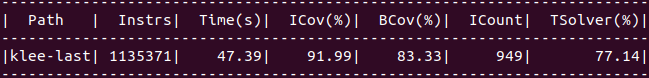
\includegraphics[scale=0.5]{TargetSearch.png}
    \caption{TargetSearch}
    \label{fig:target}
\end{figure}
\includegraphics

\noindent TargetSearch strategiju smo primenili i u slučaju kada nismo naveli sve funkcije. Kao što je već pomenuto nenavedene funkcije će biti pretražene onom strategijom koja u pozivu ima najveći broj funkcija da pretraži. Primer poziva možete videti ispod.

\begin{tcolorbox}[title={Primer poziva TargetSearch algoritma nad test fajlom}]
klee  --search=target-searcher  --target-dfs=f4,f5,f6  --target-bfs=f7 targetSearcherTest.bc 
\end{tcolorbox}
Rezultate koje smo dobili nakon poziva ove komande možete videti ovde \ref{fig:target2}

Vidimo da su dobijeni rezultati u ovom slučaju bolji nego u prethodnom slučaju. Razlog za tako nešto je to što se prilikom poziva random-path i random-state strategija pravi veliki broj stanja koja usporavaju izvršavanje algoritma.  
\begin{figure}[!htb]
    \centering
    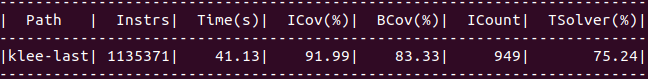
\includegraphics[scale=0.5]{TargetSearchDfsBfs.png}
    \caption{TargetSearch2}
    \label{fig:target2}
\end{figure}
\includegraphics


\noindent Naredne slike će demonstrirati dobijene rezultate koristeći algoritme koje KLEE omogućava. Za upoređivanje smo koristili dfs \ref{fig:dfs}, bfs \ref{fig:bfs}, random-state \ref{fig:rs}, random-path \ref{fig:rps}, weighted-random \ref{fig:wrs}.

\begin{figure}[!htb]
    \centering
    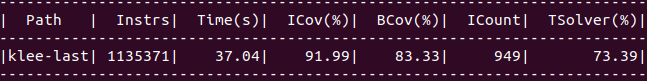
\includegraphics[scale=0.5]{dfs.png}
    \caption{DFS}
    \label{fig:dfs}
\end{figure}
\includegraphics

\begin{figure}[!htb]
    \centering
    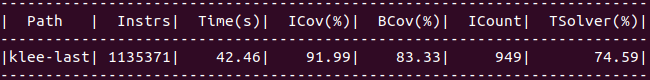
\includegraphics[scale=0.5]{bfs.png}
    \caption{BFS}
    \label{fig:bfs}
\end{figure}
\includegraphics

\begin{figure}[!htb]
    \centering
    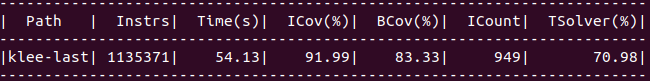
\includegraphics[scale=0.5]{rs.png}
    \caption{Random State}
    \label{fig:rs}
\end{figure}
\includegraphics

\begin{figure}[!htb]
    \centering
    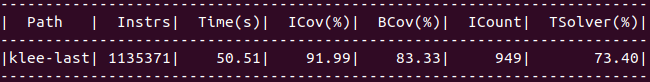
\includegraphics[scale=0.5]{rps.png}
    \caption{Random Path}
    \label{fig:rps}
\end{figure}
\includegraphics

\begin{figure}[!htb]
    \centering
    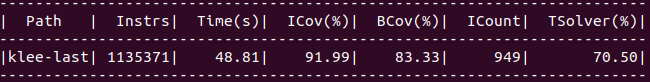
\includegraphics[scale=0.5]{wrs.png}
    \caption{Weighted Random}
    \label{fig:wrs}
\end{figure}
\includegraphics

\newpage
\noindent Kao što možemo videti na ovim slikama, naš algoritam ne daje najbolje rezultate poredeći ga sa ostalim algoritmima pretrage, zbog navedenog problema sa kreiranjem velikog broja stanja. Ipak, temeljnim testiranjem, utvrdili smo da je naš algoritam izuzetno efikasan u traženju grešaka. U takvim situacijama je bolji od svih testiranih algoritama. To su situacije u kojima je prilikom pozivanja TargetSearch algoritma navedena komanda --exit-on-error. Takođe, bitno je naglasiti da smo testiranje vršili nad funkcijama sa maksimalno dvanaest simboličkih promenljivih, jer je za veći broj izvršavanje trajalo previše dugo, pa samim tim, ne možemo ništa konkretnije reći o ponašanju našeg algoritma u takvim situacijama.


\section{Zaključak}
Algoritam TargetSearch je naša verzija strategije obilaska putanja. Ideja ja bila da se omogući odabir strategije obilaska putanja za svaku funkciju posebno u zavisnosti od toga koja strategija im najviše pogoduje, a da kao posledica toga dobijemo na efikasnosti. Efikasnost je nešto na čemu dalje može da se radi da bismo u svakoj situaciji dobili rezultate koji su bolji u poređenju sa postojećim strategijama, što sada nije slučaj.    

\newpage
\addcontentsline{toc}{section}{Literatura}
\appendix
\bibliography{TargetSearch} 
\bibliographystyle{plain}

\appendix

\end{document}
